
% Default to the notebook output style

    


% Inherit from the specified cell style.




    
\documentclass[11pt]{article}

    
    
    \usepackage[T1]{fontenc}
    % Nicer default font (+ math font) than Computer Modern for most use cases
    \usepackage{mathpazo}

    % Basic figure setup, for now with no caption control since it's done
    % automatically by Pandoc (which extracts ![](path) syntax from Markdown).
    \usepackage{graphicx}
    % We will generate all images so they have a width \maxwidth. This means
    % that they will get their normal width if they fit onto the page, but
    % are scaled down if they would overflow the margins.
    \makeatletter
    \def\maxwidth{\ifdim\Gin@nat@width>\linewidth\linewidth
    \else\Gin@nat@width\fi}
    \makeatother
    \let\Oldincludegraphics\includegraphics
    % Set max figure width to be 80% of text width, for now hardcoded.
    \renewcommand{\includegraphics}[1]{\Oldincludegraphics[width=.8\maxwidth]{#1}}
    % Ensure that by default, figures have no caption (until we provide a
    % proper Figure object with a Caption API and a way to capture that
    % in the conversion process - todo).
    \usepackage{caption}
    \DeclareCaptionLabelFormat{nolabel}{}
    \captionsetup{labelformat=nolabel}

    \usepackage{adjustbox} % Used to constrain images to a maximum size 
    \usepackage{xcolor} % Allow colors to be defined
    \usepackage{enumerate} % Needed for markdown enumerations to work
    \usepackage{geometry} % Used to adjust the document margins
    \usepackage{amsmath} % Equations
    \usepackage{amssymb} % Equations
    \usepackage{textcomp} % defines textquotesingle
    % Hack from http://tex.stackexchange.com/a/47451/13684:
    \AtBeginDocument{%
        \def\PYZsq{\textquotesingle}% Upright quotes in Pygmentized code
    }
    \usepackage{upquote} % Upright quotes for verbatim code
    \usepackage{eurosym} % defines \euro
    \usepackage[mathletters]{ucs} % Extended unicode (utf-8) support
    \usepackage[utf8x]{inputenc} % Allow utf-8 characters in the tex document
    \usepackage{fancyvrb} % verbatim replacement that allows latex
    \usepackage{grffile} % extends the file name processing of package graphics 
                         % to support a larger range 
    % The hyperref package gives us a pdf with properly built
    % internal navigation ('pdf bookmarks' for the table of contents,
    % internal cross-reference links, web links for URLs, etc.)
    \usepackage{hyperref}
    \usepackage{longtable} % longtable support required by pandoc >1.10
    \usepackage{booktabs}  % table support for pandoc > 1.12.2
    \usepackage[inline]{enumitem} % IRkernel/repr support (it uses the enumerate* environment)
    \usepackage[normalem]{ulem} % ulem is needed to support strikethroughs (\sout)
                                % normalem makes italics be italics, not underlines
    

    
    
    % Colors for the hyperref package
    \definecolor{urlcolor}{rgb}{0,.145,.698}
    \definecolor{linkcolor}{rgb}{.71,0.21,0.01}
    \definecolor{citecolor}{rgb}{.12,.54,.11}

    % ANSI colors
    \definecolor{ansi-black}{HTML}{3E424D}
    \definecolor{ansi-black-intense}{HTML}{282C36}
    \definecolor{ansi-red}{HTML}{E75C58}
    \definecolor{ansi-red-intense}{HTML}{B22B31}
    \definecolor{ansi-green}{HTML}{00A250}
    \definecolor{ansi-green-intense}{HTML}{007427}
    \definecolor{ansi-yellow}{HTML}{DDB62B}
    \definecolor{ansi-yellow-intense}{HTML}{B27D12}
    \definecolor{ansi-blue}{HTML}{208FFB}
    \definecolor{ansi-blue-intense}{HTML}{0065CA}
    \definecolor{ansi-magenta}{HTML}{D160C4}
    \definecolor{ansi-magenta-intense}{HTML}{A03196}
    \definecolor{ansi-cyan}{HTML}{60C6C8}
    \definecolor{ansi-cyan-intense}{HTML}{258F8F}
    \definecolor{ansi-white}{HTML}{C5C1B4}
    \definecolor{ansi-white-intense}{HTML}{A1A6B2}

    % commands and environments needed by pandoc snippets
    % extracted from the output of `pandoc -s`
    \providecommand{\tightlist}{%
      \setlength{\itemsep}{0pt}\setlength{\parskip}{0pt}}
    \DefineVerbatimEnvironment{Highlighting}{Verbatim}{commandchars=\\\{\}}
    % Add ',fontsize=\small' for more characters per line
    \newenvironment{Shaded}{}{}
    \newcommand{\KeywordTok}[1]{\textcolor[rgb]{0.00,0.44,0.13}{\textbf{{#1}}}}
    \newcommand{\DataTypeTok}[1]{\textcolor[rgb]{0.56,0.13,0.00}{{#1}}}
    \newcommand{\DecValTok}[1]{\textcolor[rgb]{0.25,0.63,0.44}{{#1}}}
    \newcommand{\BaseNTok}[1]{\textcolor[rgb]{0.25,0.63,0.44}{{#1}}}
    \newcommand{\FloatTok}[1]{\textcolor[rgb]{0.25,0.63,0.44}{{#1}}}
    \newcommand{\CharTok}[1]{\textcolor[rgb]{0.25,0.44,0.63}{{#1}}}
    \newcommand{\StringTok}[1]{\textcolor[rgb]{0.25,0.44,0.63}{{#1}}}
    \newcommand{\CommentTok}[1]{\textcolor[rgb]{0.38,0.63,0.69}{\textit{{#1}}}}
    \newcommand{\OtherTok}[1]{\textcolor[rgb]{0.00,0.44,0.13}{{#1}}}
    \newcommand{\AlertTok}[1]{\textcolor[rgb]{1.00,0.00,0.00}{\textbf{{#1}}}}
    \newcommand{\FunctionTok}[1]{\textcolor[rgb]{0.02,0.16,0.49}{{#1}}}
    \newcommand{\RegionMarkerTok}[1]{{#1}}
    \newcommand{\ErrorTok}[1]{\textcolor[rgb]{1.00,0.00,0.00}{\textbf{{#1}}}}
    \newcommand{\NormalTok}[1]{{#1}}
    
    % Additional commands for more recent versions of Pandoc
    \newcommand{\ConstantTok}[1]{\textcolor[rgb]{0.53,0.00,0.00}{{#1}}}
    \newcommand{\SpecialCharTok}[1]{\textcolor[rgb]{0.25,0.44,0.63}{{#1}}}
    \newcommand{\VerbatimStringTok}[1]{\textcolor[rgb]{0.25,0.44,0.63}{{#1}}}
    \newcommand{\SpecialStringTok}[1]{\textcolor[rgb]{0.73,0.40,0.53}{{#1}}}
    \newcommand{\ImportTok}[1]{{#1}}
    \newcommand{\DocumentationTok}[1]{\textcolor[rgb]{0.73,0.13,0.13}{\textit{{#1}}}}
    \newcommand{\AnnotationTok}[1]{\textcolor[rgb]{0.38,0.63,0.69}{\textbf{\textit{{#1}}}}}
    \newcommand{\CommentVarTok}[1]{\textcolor[rgb]{0.38,0.63,0.69}{\textbf{\textit{{#1}}}}}
    \newcommand{\VariableTok}[1]{\textcolor[rgb]{0.10,0.09,0.49}{{#1}}}
    \newcommand{\ControlFlowTok}[1]{\textcolor[rgb]{0.00,0.44,0.13}{\textbf{{#1}}}}
    \newcommand{\OperatorTok}[1]{\textcolor[rgb]{0.40,0.40,0.40}{{#1}}}
    \newcommand{\BuiltInTok}[1]{{#1}}
    \newcommand{\ExtensionTok}[1]{{#1}}
    \newcommand{\PreprocessorTok}[1]{\textcolor[rgb]{0.74,0.48,0.00}{{#1}}}
    \newcommand{\AttributeTok}[1]{\textcolor[rgb]{0.49,0.56,0.16}{{#1}}}
    \newcommand{\InformationTok}[1]{\textcolor[rgb]{0.38,0.63,0.69}{\textbf{\textit{{#1}}}}}
    \newcommand{\WarningTok}[1]{\textcolor[rgb]{0.38,0.63,0.69}{\textbf{\textit{{#1}}}}}
    
    
    % Define a nice break command that doesn't care if a line doesn't already
    % exist.
    \def\br{\hspace*{\fill} \\* }
    % Math Jax compatability definitions
    \def\gt{>}
    \def\lt{<}
    % Document parameters
    \title{Tutorial-2-Macquarie\_Island\_case\_study}
    
    
    

    % Pygments definitions
    
\makeatletter
\def\PY@reset{\let\PY@it=\relax \let\PY@bf=\relax%
    \let\PY@ul=\relax \let\PY@tc=\relax%
    \let\PY@bc=\relax \let\PY@ff=\relax}
\def\PY@tok#1{\csname PY@tok@#1\endcsname}
\def\PY@toks#1+{\ifx\relax#1\empty\else%
    \PY@tok{#1}\expandafter\PY@toks\fi}
\def\PY@do#1{\PY@bc{\PY@tc{\PY@ul{%
    \PY@it{\PY@bf{\PY@ff{#1}}}}}}}
\def\PY#1#2{\PY@reset\PY@toks#1+\relax+\PY@do{#2}}

\expandafter\def\csname PY@tok@w\endcsname{\def\PY@tc##1{\textcolor[rgb]{0.73,0.73,0.73}{##1}}}
\expandafter\def\csname PY@tok@c\endcsname{\let\PY@it=\textit\def\PY@tc##1{\textcolor[rgb]{0.25,0.50,0.50}{##1}}}
\expandafter\def\csname PY@tok@cp\endcsname{\def\PY@tc##1{\textcolor[rgb]{0.74,0.48,0.00}{##1}}}
\expandafter\def\csname PY@tok@k\endcsname{\let\PY@bf=\textbf\def\PY@tc##1{\textcolor[rgb]{0.00,0.50,0.00}{##1}}}
\expandafter\def\csname PY@tok@kp\endcsname{\def\PY@tc##1{\textcolor[rgb]{0.00,0.50,0.00}{##1}}}
\expandafter\def\csname PY@tok@kt\endcsname{\def\PY@tc##1{\textcolor[rgb]{0.69,0.00,0.25}{##1}}}
\expandafter\def\csname PY@tok@o\endcsname{\def\PY@tc##1{\textcolor[rgb]{0.40,0.40,0.40}{##1}}}
\expandafter\def\csname PY@tok@ow\endcsname{\let\PY@bf=\textbf\def\PY@tc##1{\textcolor[rgb]{0.67,0.13,1.00}{##1}}}
\expandafter\def\csname PY@tok@nb\endcsname{\def\PY@tc##1{\textcolor[rgb]{0.00,0.50,0.00}{##1}}}
\expandafter\def\csname PY@tok@nf\endcsname{\def\PY@tc##1{\textcolor[rgb]{0.00,0.00,1.00}{##1}}}
\expandafter\def\csname PY@tok@nc\endcsname{\let\PY@bf=\textbf\def\PY@tc##1{\textcolor[rgb]{0.00,0.00,1.00}{##1}}}
\expandafter\def\csname PY@tok@nn\endcsname{\let\PY@bf=\textbf\def\PY@tc##1{\textcolor[rgb]{0.00,0.00,1.00}{##1}}}
\expandafter\def\csname PY@tok@ne\endcsname{\let\PY@bf=\textbf\def\PY@tc##1{\textcolor[rgb]{0.82,0.25,0.23}{##1}}}
\expandafter\def\csname PY@tok@nv\endcsname{\def\PY@tc##1{\textcolor[rgb]{0.10,0.09,0.49}{##1}}}
\expandafter\def\csname PY@tok@no\endcsname{\def\PY@tc##1{\textcolor[rgb]{0.53,0.00,0.00}{##1}}}
\expandafter\def\csname PY@tok@nl\endcsname{\def\PY@tc##1{\textcolor[rgb]{0.63,0.63,0.00}{##1}}}
\expandafter\def\csname PY@tok@ni\endcsname{\let\PY@bf=\textbf\def\PY@tc##1{\textcolor[rgb]{0.60,0.60,0.60}{##1}}}
\expandafter\def\csname PY@tok@na\endcsname{\def\PY@tc##1{\textcolor[rgb]{0.49,0.56,0.16}{##1}}}
\expandafter\def\csname PY@tok@nt\endcsname{\let\PY@bf=\textbf\def\PY@tc##1{\textcolor[rgb]{0.00,0.50,0.00}{##1}}}
\expandafter\def\csname PY@tok@nd\endcsname{\def\PY@tc##1{\textcolor[rgb]{0.67,0.13,1.00}{##1}}}
\expandafter\def\csname PY@tok@s\endcsname{\def\PY@tc##1{\textcolor[rgb]{0.73,0.13,0.13}{##1}}}
\expandafter\def\csname PY@tok@sd\endcsname{\let\PY@it=\textit\def\PY@tc##1{\textcolor[rgb]{0.73,0.13,0.13}{##1}}}
\expandafter\def\csname PY@tok@si\endcsname{\let\PY@bf=\textbf\def\PY@tc##1{\textcolor[rgb]{0.73,0.40,0.53}{##1}}}
\expandafter\def\csname PY@tok@se\endcsname{\let\PY@bf=\textbf\def\PY@tc##1{\textcolor[rgb]{0.73,0.40,0.13}{##1}}}
\expandafter\def\csname PY@tok@sr\endcsname{\def\PY@tc##1{\textcolor[rgb]{0.73,0.40,0.53}{##1}}}
\expandafter\def\csname PY@tok@ss\endcsname{\def\PY@tc##1{\textcolor[rgb]{0.10,0.09,0.49}{##1}}}
\expandafter\def\csname PY@tok@sx\endcsname{\def\PY@tc##1{\textcolor[rgb]{0.00,0.50,0.00}{##1}}}
\expandafter\def\csname PY@tok@m\endcsname{\def\PY@tc##1{\textcolor[rgb]{0.40,0.40,0.40}{##1}}}
\expandafter\def\csname PY@tok@gh\endcsname{\let\PY@bf=\textbf\def\PY@tc##1{\textcolor[rgb]{0.00,0.00,0.50}{##1}}}
\expandafter\def\csname PY@tok@gu\endcsname{\let\PY@bf=\textbf\def\PY@tc##1{\textcolor[rgb]{0.50,0.00,0.50}{##1}}}
\expandafter\def\csname PY@tok@gd\endcsname{\def\PY@tc##1{\textcolor[rgb]{0.63,0.00,0.00}{##1}}}
\expandafter\def\csname PY@tok@gi\endcsname{\def\PY@tc##1{\textcolor[rgb]{0.00,0.63,0.00}{##1}}}
\expandafter\def\csname PY@tok@gr\endcsname{\def\PY@tc##1{\textcolor[rgb]{1.00,0.00,0.00}{##1}}}
\expandafter\def\csname PY@tok@ge\endcsname{\let\PY@it=\textit}
\expandafter\def\csname PY@tok@gs\endcsname{\let\PY@bf=\textbf}
\expandafter\def\csname PY@tok@gp\endcsname{\let\PY@bf=\textbf\def\PY@tc##1{\textcolor[rgb]{0.00,0.00,0.50}{##1}}}
\expandafter\def\csname PY@tok@go\endcsname{\def\PY@tc##1{\textcolor[rgb]{0.53,0.53,0.53}{##1}}}
\expandafter\def\csname PY@tok@gt\endcsname{\def\PY@tc##1{\textcolor[rgb]{0.00,0.27,0.87}{##1}}}
\expandafter\def\csname PY@tok@err\endcsname{\def\PY@bc##1{\setlength{\fboxsep}{0pt}\fcolorbox[rgb]{1.00,0.00,0.00}{1,1,1}{\strut ##1}}}
\expandafter\def\csname PY@tok@kc\endcsname{\let\PY@bf=\textbf\def\PY@tc##1{\textcolor[rgb]{0.00,0.50,0.00}{##1}}}
\expandafter\def\csname PY@tok@kd\endcsname{\let\PY@bf=\textbf\def\PY@tc##1{\textcolor[rgb]{0.00,0.50,0.00}{##1}}}
\expandafter\def\csname PY@tok@kn\endcsname{\let\PY@bf=\textbf\def\PY@tc##1{\textcolor[rgb]{0.00,0.50,0.00}{##1}}}
\expandafter\def\csname PY@tok@kr\endcsname{\let\PY@bf=\textbf\def\PY@tc##1{\textcolor[rgb]{0.00,0.50,0.00}{##1}}}
\expandafter\def\csname PY@tok@bp\endcsname{\def\PY@tc##1{\textcolor[rgb]{0.00,0.50,0.00}{##1}}}
\expandafter\def\csname PY@tok@fm\endcsname{\def\PY@tc##1{\textcolor[rgb]{0.00,0.00,1.00}{##1}}}
\expandafter\def\csname PY@tok@vc\endcsname{\def\PY@tc##1{\textcolor[rgb]{0.10,0.09,0.49}{##1}}}
\expandafter\def\csname PY@tok@vg\endcsname{\def\PY@tc##1{\textcolor[rgb]{0.10,0.09,0.49}{##1}}}
\expandafter\def\csname PY@tok@vi\endcsname{\def\PY@tc##1{\textcolor[rgb]{0.10,0.09,0.49}{##1}}}
\expandafter\def\csname PY@tok@vm\endcsname{\def\PY@tc##1{\textcolor[rgb]{0.10,0.09,0.49}{##1}}}
\expandafter\def\csname PY@tok@sa\endcsname{\def\PY@tc##1{\textcolor[rgb]{0.73,0.13,0.13}{##1}}}
\expandafter\def\csname PY@tok@sb\endcsname{\def\PY@tc##1{\textcolor[rgb]{0.73,0.13,0.13}{##1}}}
\expandafter\def\csname PY@tok@sc\endcsname{\def\PY@tc##1{\textcolor[rgb]{0.73,0.13,0.13}{##1}}}
\expandafter\def\csname PY@tok@dl\endcsname{\def\PY@tc##1{\textcolor[rgb]{0.73,0.13,0.13}{##1}}}
\expandafter\def\csname PY@tok@s2\endcsname{\def\PY@tc##1{\textcolor[rgb]{0.73,0.13,0.13}{##1}}}
\expandafter\def\csname PY@tok@sh\endcsname{\def\PY@tc##1{\textcolor[rgb]{0.73,0.13,0.13}{##1}}}
\expandafter\def\csname PY@tok@s1\endcsname{\def\PY@tc##1{\textcolor[rgb]{0.73,0.13,0.13}{##1}}}
\expandafter\def\csname PY@tok@mb\endcsname{\def\PY@tc##1{\textcolor[rgb]{0.40,0.40,0.40}{##1}}}
\expandafter\def\csname PY@tok@mf\endcsname{\def\PY@tc##1{\textcolor[rgb]{0.40,0.40,0.40}{##1}}}
\expandafter\def\csname PY@tok@mh\endcsname{\def\PY@tc##1{\textcolor[rgb]{0.40,0.40,0.40}{##1}}}
\expandafter\def\csname PY@tok@mi\endcsname{\def\PY@tc##1{\textcolor[rgb]{0.40,0.40,0.40}{##1}}}
\expandafter\def\csname PY@tok@il\endcsname{\def\PY@tc##1{\textcolor[rgb]{0.40,0.40,0.40}{##1}}}
\expandafter\def\csname PY@tok@mo\endcsname{\def\PY@tc##1{\textcolor[rgb]{0.40,0.40,0.40}{##1}}}
\expandafter\def\csname PY@tok@ch\endcsname{\let\PY@it=\textit\def\PY@tc##1{\textcolor[rgb]{0.25,0.50,0.50}{##1}}}
\expandafter\def\csname PY@tok@cm\endcsname{\let\PY@it=\textit\def\PY@tc##1{\textcolor[rgb]{0.25,0.50,0.50}{##1}}}
\expandafter\def\csname PY@tok@cpf\endcsname{\let\PY@it=\textit\def\PY@tc##1{\textcolor[rgb]{0.25,0.50,0.50}{##1}}}
\expandafter\def\csname PY@tok@c1\endcsname{\let\PY@it=\textit\def\PY@tc##1{\textcolor[rgb]{0.25,0.50,0.50}{##1}}}
\expandafter\def\csname PY@tok@cs\endcsname{\let\PY@it=\textit\def\PY@tc##1{\textcolor[rgb]{0.25,0.50,0.50}{##1}}}

\def\PYZbs{\char`\\}
\def\PYZus{\char`\_}
\def\PYZob{\char`\{}
\def\PYZcb{\char`\}}
\def\PYZca{\char`\^}
\def\PYZam{\char`\&}
\def\PYZlt{\char`\<}
\def\PYZgt{\char`\>}
\def\PYZsh{\char`\#}
\def\PYZpc{\char`\%}
\def\PYZdl{\char`\$}
\def\PYZhy{\char`\-}
\def\PYZsq{\char`\'}
\def\PYZdq{\char`\"}
\def\PYZti{\char`\~}
% for compatibility with earlier versions
\def\PYZat{@}
\def\PYZlb{[}
\def\PYZrb{]}
\makeatother


    % Exact colors from NB
    \definecolor{incolor}{rgb}{0.0, 0.0, 0.5}
    \definecolor{outcolor}{rgb}{0.545, 0.0, 0.0}



    
    % Prevent overflowing lines due to hard-to-break entities
    \sloppy 
    % Setup hyperref package
    \hypersetup{
      breaklinks=true,  % so long urls are correctly broken across lines
      colorlinks=true,
      urlcolor=urlcolor,
      linkcolor=linkcolor,
      citecolor=citecolor,
      }
    % Slightly bigger margins than the latex defaults
    
    \geometry{verbose,tmargin=1in,bmargin=1in,lmargin=1in,rmargin=1in}
    
    

    \begin{document}
    
    
    \maketitle
    
    

    
    We define the Macquarie Island interaction network by the species
present, the interactions between them, and the signs of these
interactions. The network structure is encoded as a \texttt{networkx}
digraph. The function \texttt{initialise\_foodweb} stores the signs of
the interactions in the edge data dictionary. The network can be drawn
using \texttt{draw\_foodweb}.

    \begin{Verbatim}[commandchars=\\\{\}]
{\color{incolor}In [{\color{incolor}90}]:} \PY{k+kn}{from} \PY{n+nn}{qualmod} \PY{k}{import} \PY{n}{initialise\PYZus{}foodweb}\PY{p}{,} \PY{n}{draw\PYZus{}foodweb}
         \PY{k+kn}{from} \PY{n+nn}{qualmod} \PY{k}{import} \PY{n}{qualitative\PYZus{}community\PYZus{}matrix}\PY{p}{,} \PY{n}{get\PYZus{}conditions\PYZus{}lists}
         \PY{k+kn}{import} \PY{n+nn}{numpy} \PY{k}{as} \PY{n+nn}{np}
         \PY{k+kn}{import} \PY{n+nn}{time}
         
         \PY{k+kn}{from} \PY{n+nn}{IPython}\PY{n+nn}{.}\PY{n+nn}{display} \PY{k}{import} \PY{n}{Image}
         \PY{k+kn}{import} \PY{n+nn}{os}
         
         \PY{n}{sppList} \PY{o}{=} \PY{p}{[} 
             \PY{l+s+s1}{\PYZsq{}}\PY{l+s+s1}{albatrosses}\PY{l+s+s1}{\PYZsq{}}\PY{p}{,}
             \PY{l+s+s1}{\PYZsq{}}\PY{l+s+s1}{prions}\PY{l+s+s1}{\PYZsq{}}\PY{p}{,}
             \PY{l+s+s1}{\PYZsq{}}\PY{l+s+s1}{burrowSeabirds}\PY{l+s+s1}{\PYZsq{}}\PY{p}{,}
             \PY{l+s+s1}{\PYZsq{}}\PY{l+s+s1}{petrels}\PY{l+s+s1}{\PYZsq{}}\PY{p}{,}
             \PY{l+s+s1}{\PYZsq{}}\PY{l+s+s1}{herbfield}\PY{l+s+s1}{\PYZsq{}}\PY{p}{,}
             \PY{l+s+s1}{\PYZsq{}}\PY{l+s+s1}{macroInverts}\PY{l+s+s1}{\PYZsq{}}\PY{p}{,}
             \PY{l+s+s1}{\PYZsq{}}\PY{l+s+s1}{mice}\PY{l+s+s1}{\PYZsq{}}\PY{p}{,}
             \PY{l+s+s1}{\PYZsq{}}\PY{l+s+s1}{penguins}\PY{l+s+s1}{\PYZsq{}}\PY{p}{,}
             \PY{l+s+s1}{\PYZsq{}}\PY{l+s+s1}{rabbits}\PY{l+s+s1}{\PYZsq{}}\PY{p}{,}
             \PY{l+s+s1}{\PYZsq{}}\PY{l+s+s1}{rats}\PY{l+s+s1}{\PYZsq{}}\PY{p}{,}
             \PY{l+s+s1}{\PYZsq{}}\PY{l+s+s1}{redpolls}\PY{l+s+s1}{\PYZsq{}}\PY{p}{,}
             \PY{l+s+s1}{\PYZsq{}}\PY{l+s+s1}{skuas}\PY{l+s+s1}{\PYZsq{}}\PY{p}{,}
             \PY{l+s+s1}{\PYZsq{}}\PY{l+s+s1}{surfaceSeabirds}\PY{l+s+s1}{\PYZsq{}}\PY{p}{,}
             \PY{l+s+s1}{\PYZsq{}}\PY{l+s+s1}{tussock}\PY{l+s+s1}{\PYZsq{}}\PY{p}{,}
         \PY{p}{]}
         
         \PY{c+c1}{\PYZsh{} key is recipient of positive effect}
         \PY{n}{positive\PYZus{}edges\PYZus{}dict} \PY{o}{=} \PY{p}{\PYZob{}}
             \PY{l+s+s1}{\PYZsq{}}\PY{l+s+s1}{prions}\PY{l+s+s1}{\PYZsq{}}\PY{p}{:}           \PY{p}{[}\PY{l+s+s1}{\PYZsq{}}\PY{l+s+s1}{grassland}\PY{l+s+s1}{\PYZsq{}}\PY{p}{]}\PY{p}{,}
             \PY{l+s+s1}{\PYZsq{}}\PY{l+s+s1}{skuas}\PY{l+s+s1}{\PYZsq{}}\PY{p}{:}            \PY{p}{[}\PY{l+s+s1}{\PYZsq{}}\PY{l+s+s1}{prions}\PY{l+s+s1}{\PYZsq{}}\PY{p}{,}\PY{l+s+s1}{\PYZsq{}}\PY{l+s+s1}{burrowSeabirds}\PY{l+s+s1}{\PYZsq{}}\PY{p}{,}\PY{l+s+s1}{\PYZsq{}}\PY{l+s+s1}{rabbits}\PY{l+s+s1}{\PYZsq{}}\PY{p}{,}\PY{l+s+s1}{\PYZsq{}}\PY{l+s+s1}{penguins}\PY{l+s+s1}{\PYZsq{}}\PY{p}{]}\PY{p}{,}
             \PY{l+s+s1}{\PYZsq{}}\PY{l+s+s1}{petrels}\PY{l+s+s1}{\PYZsq{}}\PY{p}{:}          \PY{p}{[}\PY{l+s+s1}{\PYZsq{}}\PY{l+s+s1}{penguins}\PY{l+s+s1}{\PYZsq{}}\PY{p}{,}\PY{l+s+s1}{\PYZsq{}}\PY{l+s+s1}{tussock}\PY{l+s+s1}{\PYZsq{}}\PY{p}{,}\PY{l+s+s1}{\PYZsq{}}\PY{l+s+s1}{grassland}\PY{l+s+s1}{\PYZsq{}}\PY{p}{]}\PY{p}{,}
             \PY{l+s+s1}{\PYZsq{}}\PY{l+s+s1}{mice}\PY{l+s+s1}{\PYZsq{}}\PY{p}{:}             \PY{p}{[}\PY{l+s+s1}{\PYZsq{}}\PY{l+s+s1}{herbfield}\PY{l+s+s1}{\PYZsq{}}\PY{p}{,}\PY{l+s+s1}{\PYZsq{}}\PY{l+s+s1}{macroInverts}\PY{l+s+s1}{\PYZsq{}}\PY{p}{,}\PY{l+s+s1}{\PYZsq{}}\PY{l+s+s1}{tussock}\PY{l+s+s1}{\PYZsq{}}\PY{p}{]}\PY{p}{,}
             \PY{l+s+s1}{\PYZsq{}}\PY{l+s+s1}{rats}\PY{l+s+s1}{\PYZsq{}}\PY{p}{:}             \PY{p}{[}\PY{l+s+s1}{\PYZsq{}}\PY{l+s+s1}{macroInverts}\PY{l+s+s1}{\PYZsq{}}\PY{p}{,}\PY{l+s+s1}{\PYZsq{}}\PY{l+s+s1}{herbfield}\PY{l+s+s1}{\PYZsq{}}\PY{p}{,}\PY{l+s+s1}{\PYZsq{}}\PY{l+s+s1}{tussock}\PY{l+s+s1}{\PYZsq{}}\PY{p}{]}\PY{p}{,}
             \PY{l+s+s1}{\PYZsq{}}\PY{l+s+s1}{burrowSeabirds}\PY{l+s+s1}{\PYZsq{}}\PY{p}{:}   \PY{p}{[}\PY{l+s+s1}{\PYZsq{}}\PY{l+s+s1}{tussock}\PY{l+s+s1}{\PYZsq{}}\PY{p}{]}\PY{p}{,}
             \PY{l+s+s1}{\PYZsq{}}\PY{l+s+s1}{rabbits}\PY{l+s+s1}{\PYZsq{}}\PY{p}{:}          \PY{p}{[}\PY{l+s+s1}{\PYZsq{}}\PY{l+s+s1}{tussock}\PY{l+s+s1}{\PYZsq{}}\PY{p}{,}\PY{l+s+s1}{\PYZsq{}}\PY{l+s+s1}{herbfield}\PY{l+s+s1}{\PYZsq{}}\PY{p}{,}\PY{l+s+s1}{\PYZsq{}}\PY{l+s+s1}{grassland}\PY{l+s+s1}{\PYZsq{}}\PY{p}{]}\PY{p}{,}
             \PY{l+s+s1}{\PYZsq{}}\PY{l+s+s1}{macroInverts}\PY{l+s+s1}{\PYZsq{}}\PY{p}{:}     \PY{p}{[}\PY{l+s+s1}{\PYZsq{}}\PY{l+s+s1}{herbfield}\PY{l+s+s1}{\PYZsq{}}\PY{p}{,}\PY{l+s+s1}{\PYZsq{}}\PY{l+s+s1}{grassland}\PY{l+s+s1}{\PYZsq{}}\PY{p}{,}\PY{l+s+s1}{\PYZsq{}}\PY{l+s+s1}{tussock}\PY{l+s+s1}{\PYZsq{}}\PY{p}{]}\PY{p}{,}
             \PY{l+s+s1}{\PYZsq{}}\PY{l+s+s1}{albatrosses}\PY{l+s+s1}{\PYZsq{}}\PY{p}{:}      \PY{p}{[}\PY{l+s+s1}{\PYZsq{}}\PY{l+s+s1}{tussock}\PY{l+s+s1}{\PYZsq{}}\PY{p}{,}\PY{l+s+s1}{\PYZsq{}}\PY{l+s+s1}{herbfield}\PY{l+s+s1}{\PYZsq{}}\PY{p}{]}\PY{p}{,}
             \PY{l+s+s1}{\PYZsq{}}\PY{l+s+s1}{redpolls}\PY{l+s+s1}{\PYZsq{}}\PY{p}{:}         \PY{p}{[}\PY{l+s+s1}{\PYZsq{}}\PY{l+s+s1}{macroInverts}\PY{l+s+s1}{\PYZsq{}}\PY{p}{,}\PY{l+s+s1}{\PYZsq{}}\PY{l+s+s1}{tussock}\PY{l+s+s1}{\PYZsq{}}\PY{p}{,}\PY{l+s+s1}{\PYZsq{}}\PY{l+s+s1}{herbfield}\PY{l+s+s1}{\PYZsq{}}\PY{p}{,}\PY{l+s+s1}{\PYZsq{}}\PY{l+s+s1}{grassland}\PY{l+s+s1}{\PYZsq{}}\PY{p}{]}\PY{p}{,}
         \PY{p}{\PYZcb{}}
         \PY{n}{negative\PYZus{}edges\PYZus{}dict} \PY{o}{=} \PY{p}{\PYZob{}}
             \PY{l+s+s1}{\PYZsq{}}\PY{l+s+s1}{prions}\PY{l+s+s1}{\PYZsq{}}\PY{p}{:}           \PY{p}{[}\PY{l+s+s1}{\PYZsq{}}\PY{l+s+s1}{prions}\PY{l+s+s1}{\PYZsq{}}\PY{p}{,}\PY{l+s+s1}{\PYZsq{}}\PY{l+s+s1}{skuas}\PY{l+s+s1}{\PYZsq{}}\PY{p}{]}\PY{p}{,}
             \PY{l+s+s1}{\PYZsq{}}\PY{l+s+s1}{skuas}\PY{l+s+s1}{\PYZsq{}}\PY{p}{:}            \PY{p}{[}\PY{l+s+s1}{\PYZsq{}}\PY{l+s+s1}{skuas}\PY{l+s+s1}{\PYZsq{}}\PY{p}{,}\PY{l+s+s1}{\PYZsq{}}\PY{l+s+s1}{tussock}\PY{l+s+s1}{\PYZsq{}}\PY{p}{]}\PY{p}{,}
             \PY{l+s+s1}{\PYZsq{}}\PY{l+s+s1}{penguins}\PY{l+s+s1}{\PYZsq{}}\PY{p}{:}         \PY{p}{[}\PY{l+s+s1}{\PYZsq{}}\PY{l+s+s1}{penguins}\PY{l+s+s1}{\PYZsq{}}\PY{p}{,}\PY{l+s+s1}{\PYZsq{}}\PY{l+s+s1}{skuas}\PY{l+s+s1}{\PYZsq{}}\PY{p}{,}\PY{l+s+s1}{\PYZsq{}}\PY{l+s+s1}{petrels}\PY{l+s+s1}{\PYZsq{}}\PY{p}{]}\PY{p}{,}
             \PY{l+s+s1}{\PYZsq{}}\PY{l+s+s1}{petrels}\PY{l+s+s1}{\PYZsq{}}\PY{p}{:}          \PY{p}{[}\PY{l+s+s1}{\PYZsq{}}\PY{l+s+s1}{petrels}\PY{l+s+s1}{\PYZsq{}}\PY{p}{]}\PY{p}{,}
             \PY{l+s+s1}{\PYZsq{}}\PY{l+s+s1}{mice}\PY{l+s+s1}{\PYZsq{}}\PY{p}{:}             \PY{p}{[}\PY{l+s+s1}{\PYZsq{}}\PY{l+s+s1}{mice}\PY{l+s+s1}{\PYZsq{}}\PY{p}{,}\PY{l+s+s1}{\PYZsq{}}\PY{l+s+s1}{rats}\PY{l+s+s1}{\PYZsq{}}\PY{p}{]}\PY{p}{,}
             \PY{l+s+s1}{\PYZsq{}}\PY{l+s+s1}{rats}\PY{l+s+s1}{\PYZsq{}}\PY{p}{:}             \PY{p}{[}\PY{l+s+s1}{\PYZsq{}}\PY{l+s+s1}{rats}\PY{l+s+s1}{\PYZsq{}}\PY{p}{]}\PY{p}{,}
             \PY{l+s+s1}{\PYZsq{}}\PY{l+s+s1}{burrowSeabirds}\PY{l+s+s1}{\PYZsq{}}\PY{p}{:}   \PY{p}{[}\PY{l+s+s1}{\PYZsq{}}\PY{l+s+s1}{burrowSeabirds}\PY{l+s+s1}{\PYZsq{}}\PY{p}{,}\PY{l+s+s1}{\PYZsq{}}\PY{l+s+s1}{skuas}\PY{l+s+s1}{\PYZsq{}}\PY{p}{,}\PY{l+s+s1}{\PYZsq{}}\PY{l+s+s1}{rabbits}\PY{l+s+s1}{\PYZsq{}}\PY{p}{]}\PY{p}{,}
             \PY{l+s+s1}{\PYZsq{}}\PY{l+s+s1}{rabbits}\PY{l+s+s1}{\PYZsq{}}\PY{p}{:}          \PY{p}{[}\PY{l+s+s1}{\PYZsq{}}\PY{l+s+s1}{rabbits}\PY{l+s+s1}{\PYZsq{}}\PY{p}{,}\PY{l+s+s1}{\PYZsq{}}\PY{l+s+s1}{skuas}\PY{l+s+s1}{\PYZsq{}}\PY{p}{]}\PY{p}{,}
             \PY{l+s+s1}{\PYZsq{}}\PY{l+s+s1}{surfaceSeabirds}\PY{l+s+s1}{\PYZsq{}}\PY{p}{:}  \PY{p}{[}\PY{l+s+s1}{\PYZsq{}}\PY{l+s+s1}{surfaceSeabirds}\PY{l+s+s1}{\PYZsq{}}\PY{p}{,}\PY{l+s+s1}{\PYZsq{}}\PY{l+s+s1}{rats}\PY{l+s+s1}{\PYZsq{}}\PY{p}{]}\PY{p}{,}
             \PY{l+s+s1}{\PYZsq{}}\PY{l+s+s1}{macroInverts}\PY{l+s+s1}{\PYZsq{}}\PY{p}{:}     \PY{p}{[}\PY{l+s+s1}{\PYZsq{}}\PY{l+s+s1}{macroInverts}\PY{l+s+s1}{\PYZsq{}}\PY{p}{,}\PY{l+s+s1}{\PYZsq{}}\PY{l+s+s1}{rats}\PY{l+s+s1}{\PYZsq{}}\PY{p}{,}\PY{l+s+s1}{\PYZsq{}}\PY{l+s+s1}{mice}\PY{l+s+s1}{\PYZsq{}}\PY{p}{,}\PY{l+s+s1}{\PYZsq{}}\PY{l+s+s1}{redpolls}\PY{l+s+s1}{\PYZsq{}}\PY{p}{]}\PY{p}{,}
             \PY{l+s+s1}{\PYZsq{}}\PY{l+s+s1}{tussock}\PY{l+s+s1}{\PYZsq{}}\PY{p}{:}          \PY{p}{[}\PY{l+s+s1}{\PYZsq{}}\PY{l+s+s1}{tussock}\PY{l+s+s1}{\PYZsq{}}\PY{p}{,}\PY{l+s+s1}{\PYZsq{}}\PY{l+s+s1}{mice}\PY{l+s+s1}{\PYZsq{}}\PY{p}{,}\PY{l+s+s1}{\PYZsq{}}\PY{l+s+s1}{rats}\PY{l+s+s1}{\PYZsq{}}\PY{p}{,}\PY{l+s+s1}{\PYZsq{}}\PY{l+s+s1}{rabbits}\PY{l+s+s1}{\PYZsq{}}\PY{p}{]}\PY{p}{,}
             \PY{l+s+s1}{\PYZsq{}}\PY{l+s+s1}{albatrosses}\PY{l+s+s1}{\PYZsq{}}\PY{p}{:}      \PY{p}{[}\PY{l+s+s1}{\PYZsq{}}\PY{l+s+s1}{albatrosses}\PY{l+s+s1}{\PYZsq{}}\PY{p}{]}\PY{p}{,}
             \PY{l+s+s1}{\PYZsq{}}\PY{l+s+s1}{herbfield}\PY{l+s+s1}{\PYZsq{}}\PY{p}{:}        \PY{p}{[}\PY{l+s+s1}{\PYZsq{}}\PY{l+s+s1}{herbfield}\PY{l+s+s1}{\PYZsq{}}\PY{p}{,}\PY{l+s+s1}{\PYZsq{}}\PY{l+s+s1}{rabbits}\PY{l+s+s1}{\PYZsq{}}\PY{p}{]}\PY{p}{,}
             \PY{l+s+s1}{\PYZsq{}}\PY{l+s+s1}{grassland}\PY{l+s+s1}{\PYZsq{}}\PY{p}{:}        \PY{p}{[}\PY{l+s+s1}{\PYZsq{}}\PY{l+s+s1}{grassland}\PY{l+s+s1}{\PYZsq{}}\PY{p}{]}\PY{p}{,}
             \PY{l+s+s1}{\PYZsq{}}\PY{l+s+s1}{redpolls}\PY{l+s+s1}{\PYZsq{}}\PY{p}{:}         \PY{p}{[}\PY{l+s+s1}{\PYZsq{}}\PY{l+s+s1}{redpolls}\PY{l+s+s1}{\PYZsq{}}\PY{p}{]}\PY{p}{,}
         \PY{p}{\PYZcb{}}
         
         \PY{n}{web} \PY{o}{=} \PY{n}{initialise\PYZus{}foodweb}\PY{p}{(}\PY{n}{positive\PYZus{}edges\PYZus{}dict}\PY{p}{,} \PY{n}{negative\PYZus{}edges\PYZus{}dict}\PY{p}{)}
         
         \PY{n}{draw\PYZus{}foodweb}\PY{p}{(}\PY{n}{web}\PY{p}{,} \PY{n}{f\PYZus{}name} \PY{o}{=} \PY{l+s+s1}{\PYZsq{}}\PY{l+s+s1}{macq1.dot}\PY{l+s+s1}{\PYZsq{}}\PY{p}{)}
         \PY{c+c1}{\PYZsh{} call graphviz to create a png, display in markdown cell}
         \PY{n}{os}\PY{o}{.}\PY{n}{system}\PY{p}{(}\PY{l+s+s2}{\PYZdq{}}\PY{l+s+s2}{dot \PYZhy{}Tpng macq1.dot \PYZgt{} macq1.png}\PY{l+s+s2}{\PYZdq{}}\PY{p}{)}
\end{Verbatim}


\begin{Verbatim}[commandchars=\\\{\}]
{\color{outcolor}Out[{\color{outcolor}90}]:} 0
\end{Verbatim}
            
    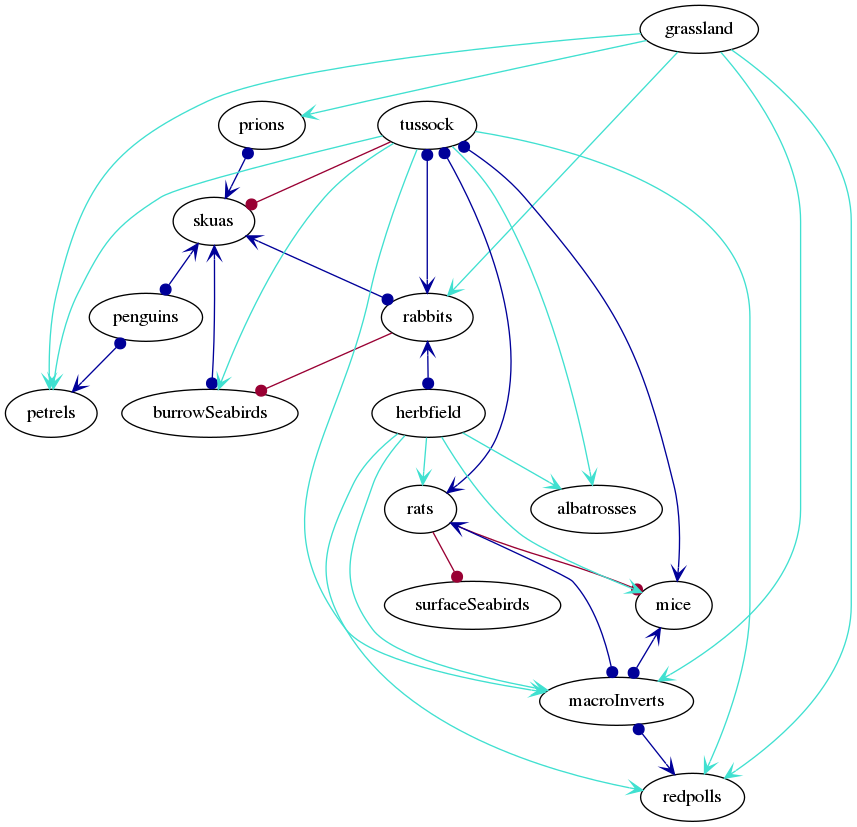
\includegraphics{macq1.png} Macquarie Island interaction network.

    We encode the validation criteria (with respect to a positive
perturbation of the rabbits).

    \begin{Verbatim}[commandchars=\\\{\}]
{\color{incolor}In [{\color{incolor}74}]:} \PY{n}{control\PYZus{}list} \PY{o}{=} \PY{p}{[}\PY{l+s+s1}{\PYZsq{}}\PY{l+s+s1}{rabbits}\PY{l+s+s1}{\PYZsq{}}\PY{p}{]} 
         
         \PY{c+c1}{\PYZsh{} Reponse to increase in rabbits}
         \PY{n}{validation} \PY{o}{=} \PY{p}{\PYZob{}}
             \PY{l+s+s1}{\PYZsq{}}\PY{l+s+s1}{rabbits}\PY{l+s+s1}{\PYZsq{}}\PY{p}{:} \PY{o}{+}\PY{l+m+mi}{1}\PY{p}{,}          
             \PY{l+s+s1}{\PYZsq{}}\PY{l+s+s1}{tussock}\PY{l+s+s1}{\PYZsq{}}\PY{p}{:} \PY{o}{\PYZhy{}}\PY{l+m+mi}{1}\PY{p}{,}
         \PY{p}{\PYZcb{}}     
\end{Verbatim}


    We convert the interaction network into a qualitative community matrix,
\texttt{Mq} below, using the function
\texttt{qualitative\_community\_matrix}.

    \begin{Verbatim}[commandchars=\\\{\}]
{\color{incolor}In [{\color{incolor}78}]:} \PY{n}{sz} \PY{o}{=} \PY{n}{web}\PY{o}{.}\PY{n}{order}\PY{p}{(}\PY{p}{)}
         \PY{p}{(}\PY{n}{Mq}\PY{p}{,} \PY{n}{s2idx}\PY{p}{)} \PY{o}{=} \PY{n}{qualitative\PYZus{}community\PYZus{}matrix}\PY{p}{(}\PY{n}{web}\PY{p}{)}
         \PY{n+nb}{print}\PY{p}{(}\PY{n}{Mq}\PY{p}{)}
\end{Verbatim}


    \begin{Verbatim}[commandchars=\\\{\}]
[[-1.  0.  0.  1.  0.  0.  0.  0.  0.  0.  0.  0.  0.  0.  1.]
 [ 0. -1.  0.  0.  0.  0.  0.  0.  0. -1.  0.  0. -1.  0.  1.]
 [ 0.  0. -1.  0.  0.  0.  0.  0.  0.  0.  0.  0.  0.  0.  0.]
 [ 0.  0.  0. -1.  0.  0.  0.  0.  0. -1.  0.  0.  0.  0.  0.]
 [ 0.  0.  1.  1. -1. -1.  0.  0.  0.  0. -1. -1.  0.  0.  1.]
 [ 0.  0.  0.  1.  1. -1.  0.  0.  0.  0. -1.  0.  0.  0.  1.]
 [ 0.  0.  0.  0.  0.  0. -1. -1.  0.  0.  0.  0. -1.  0.  0.]
 [ 0.  0.  1.  0.  0.  0.  1. -1.  0.  0.  0.  0.  0.  0.  1.]
 [ 0.  0.  1.  0.  0.  0.  0.  0. -1.  0.  0.  0. -1.  0.  0.]
 [ 0.  0.  1.  1.  0.  0.  0.  0.  0. -1.  0.  0. -1.  0.  1.]
 [ 0.  0.  0.  1.  1.  0.  0.  0.  0.  0. -1.  0.  0.  0.  1.]
 [ 0.  0.  1.  1.  1.  0.  0.  0.  0.  0.  0. -1.  0.  0.  1.]
 [ 0.  1.  0.  0.  0.  0.  1.  0.  1.  1.  0.  0. -1.  0. -1.]
 [ 0.  0.  0.  0.  0.  0.  0.  0.  0.  0. -1.  0.  0. -1.  0.]
 [ 0.  0.  0.  0.  0. -1.  0.  0.  0. -1. -1.  0.  0.  0. -1.]]

    \end{Verbatim}

    The \texttt{s2idx} returned is a bidirection dictionary that maps the
name of the species to their index in the qualitative community matrix

    \begin{Verbatim}[commandchars=\\\{\}]
{\color{incolor}In [{\color{incolor}79}]:} \PY{n}{s2idx}\PY{o}{.}\PY{n}{inv}\PY{p}{[}\PY{l+m+mi}{9}\PY{p}{]}
\end{Verbatim}


\begin{Verbatim}[commandchars=\\\{\}]
{\color{outcolor}Out[{\color{outcolor}79}]:} 'rabbits'
\end{Verbatim}
            
    The validation conditions with respect to the indices of the qualitative
matrix can be obtained using the function
\texttt{get\_conditions\_list}.

    \begin{Verbatim}[commandchars=\\\{\}]
{\color{incolor}In [{\color{incolor}77}]:} \PY{c+c1}{\PYZsh{} validation condition}
         \PY{n}{condn\PYZus{}idxs}\PY{p}{,} \PY{n}{condn} \PY{o}{=} \PY{n}{get\PYZus{}conditions\PYZus{}lists}\PY{p}{(}\PY{n}{s2idx}\PY{p}{,} \PY{n}{validation}\PY{p}{)}
         
         \PY{n+nb}{print}\PY{p}{(}\PY{n+nb}{list}\PY{p}{(}\PY{n+nb}{zip}\PY{p}{(}\PY{n}{condn\PYZus{}idxs}\PY{p}{,} \PY{n}{condn}\PY{p}{)}\PY{p}{)}\PY{p}{)}
\end{Verbatim}


    \begin{Verbatim}[commandchars=\\\{\}]
[(9, 1), (14, -1)]

    \end{Verbatim}

    To save time in this tutorial, I have hard-coded in the number of
species-response combinations to be found, which is 36. If you do not
know what the number is beforehand, you would use a line similar to the
one commented-out above the start of the \texttt{while} loop.

The \texttt{while} loop collects species response combinations using a
parameter-value sweep of the model.

    \begin{Verbatim}[commandchars=\\\{\}]
{\color{incolor}In [{\color{incolor}91}]:} \PY{c+c1}{\PYZsh{} Initialise collected responses with empty sets}
         \PY{c+c1}{\PYZsh{} Key is species perturbed and set will contain tuples of responses}
         \PY{n}{collectedResponses} \PY{o}{=} \PY{p}{\PYZob{}}\PY{n}{spp}\PY{p}{:} \PY{n+nb}{set}\PY{p}{(}\PY{p}{)} \PY{k}{for} \PY{n}{spp} \PY{o+ow}{in} \PY{n}{control\PYZus{}list}\PY{p}{\PYZcb{}} 
         
         \PY{n}{t} \PY{o}{=} \PY{l+m+mi}{1}
         \PY{n}{t\PYZus{}last\PYZus{}updated} \PY{o}{=} \PY{l+m+mi}{0}
         \PY{n}{start\PYZus{}time} \PY{o}{=} \PY{n}{time}\PY{o}{.}\PY{n}{time}\PY{p}{(}\PY{p}{)}
         
         \PY{c+c1}{\PYZsh{} use something like this if you don\PYZsq{}t }
         \PY{c+c1}{\PYZsh{} know the answer beforehand \PYZti{} 10 minutes}
         \PY{c+c1}{\PYZsh{} while t \PYZlt{} 1e6: }
         
         \PY{c+c1}{\PYZsh{} I know there are 36 responses to find}
         \PY{k}{while} \PY{n+nb}{len}\PY{p}{(}\PY{n}{collectedResponses}\PY{p}{[}\PY{l+s+s1}{\PYZsq{}}\PY{l+s+s1}{rabbits}\PY{l+s+s1}{\PYZsq{}}\PY{p}{]}\PY{p}{)} \PY{o}{\PYZlt{}} \PY{l+m+mi}{36}\PY{p}{:}
             
             
             \PY{c+c1}{\PYZsh{} Find valid stable community matrix}
             \PY{n}{valid} \PY{o}{=} \PY{k+kc}{False}
         
             \PY{k}{while} \PY{o+ow}{not} \PY{n}{valid}\PY{p}{:}
             
                 \PY{c+c1}{\PYZsh{} Find a random community matrix that is stable}
                 \PY{n}{maxEig} \PY{o}{=} \PY{l+m+mi}{1}
         
                 \PY{k}{while} \PY{n}{maxEig} \PY{o}{\PYZgt{}} \PY{l+m+mi}{0}\PY{p}{:}
                     \PY{n}{M} \PY{o}{=} \PY{n}{np}\PY{o}{.}\PY{n}{multiply}\PY{p}{(}\PY{n}{np}\PY{o}{.}\PY{n}{random}\PY{o}{.}\PY{n}{random\PYZus{}sample}\PY{p}{(}\PY{p}{(}\PY{n}{sz}\PY{p}{,}\PY{n}{sz}\PY{p}{)}\PY{p}{)}\PY{p}{,} \PY{n}{Mq}\PY{p}{)}
                     \PY{n}{maxEig} \PY{o}{=} \PY{n+nb}{max}\PY{p}{(}\PY{n}{np}\PY{o}{.}\PY{n}{real}\PY{p}{(}\PY{n}{np}\PY{o}{.}\PY{n}{linalg}\PY{o}{.}\PY{n}{eigvals}\PY{p}{(}\PY{n}{M}\PY{p}{)}\PY{p}{)}\PY{p}{)}
         
                 \PY{c+c1}{\PYZsh{} Now have a stable matrix}
         
                 \PY{c+c1}{\PYZsh{} Find sensitivity matrix}
                 \PY{n}{Sq} \PY{o}{=} \PY{o}{\PYZhy{}} \PY{n}{np}\PY{o}{.}\PY{n}{linalg}\PY{o}{.}\PY{n}{inv}\PY{p}{(}\PY{n}{M}\PY{p}{)}
         
                 \PY{c+c1}{\PYZsh{} Check validation criteria}
                 \PY{n}{valid} \PY{o}{=} \PY{n+nb}{all}\PY{p}{(}\PY{n}{np}\PY{o}{.}\PY{n}{sign}\PY{p}{(}\PY{n}{Sq}\PY{p}{[}\PY{n}{condn\PYZus{}idxs}\PY{p}{,}\PY{n}{s2idx}\PY{p}{[}\PY{l+s+s1}{\PYZsq{}}\PY{l+s+s1}{rabbits}\PY{l+s+s1}{\PYZsq{}}\PY{p}{]}\PY{p}{]}\PY{p}{)} \PY{o}{==} \PY{n}{condn}\PY{p}{)}
         
             \PY{c+c1}{\PYZsh{} Now have a valid stable community matrix}
         
             \PY{k}{for} \PY{n}{ps} \PY{o+ow}{in} \PY{n}{control\PYZus{}list}\PY{p}{:}
         
                 \PY{c+c1}{\PYZsh{} NOTE: looking at increase in rabbits not decrease here}
                 \PY{n}{response} \PY{o}{=} \PY{n+nb}{tuple}\PY{p}{(}\PY{l+s+s1}{\PYZsq{}}\PY{l+s+s1}{neg}\PY{l+s+s1}{\PYZsq{}} \PY{k}{if} \PY{n}{Sq}\PY{p}{[}\PY{n}{s2idx}\PY{p}{[}\PY{n}{ms}\PY{p}{]}\PY{p}{,}\PY{n}{s2idx}\PY{p}{[}\PY{n}{ps}\PY{p}{]}\PY{p}{]}\PY{o}{\PYZlt{}}\PY{l+m+mi}{0} \PY{k}{else} \PY{l+s+s1}{\PYZsq{}}\PY{l+s+s1}{pos}\PY{l+s+s1}{\PYZsq{}} 
                                  \PY{k}{if} \PY{n}{Sq}\PY{p}{[}\PY{n}{s2idx}\PY{p}{[}\PY{n}{ms}\PY{p}{]}\PY{p}{,}\PY{n}{s2idx}\PY{p}{[}\PY{n}{ps}\PY{p}{]}\PY{p}{]}\PY{o}{\PYZgt{}}\PY{l+m+mi}{0} \PY{k}{else} \PY{l+s+s1}{\PYZsq{}}\PY{l+s+s1}{zer}\PY{l+s+s1}{\PYZsq{}} 
                                  \PY{k}{for} \PY{n}{ms} \PY{o+ow}{in} \PY{n}{sppList}\PY{p}{)}
         
                 \PY{k}{if} \PY{n}{response} \PY{o+ow}{not} \PY{o+ow}{in} \PY{n}{collectedResponses}\PY{p}{[}\PY{n}{ps}\PY{p}{]}\PY{p}{:}
         
                     \PY{c+c1}{\PYZsh{} fs[ps].write(\PYZsq{},\PYZsq{}.join(response) + \PYZsq{}\PYZbs{}n\PYZsq{})}
                     \PY{n}{collectedResponses}\PY{p}{[}\PY{n}{ps}\PY{p}{]}\PY{o}{.}\PY{n}{add}\PY{p}{(}\PY{n}{response}\PY{p}{)}
                     \PY{n}{t\PYZus{}last\PYZus{}updated} \PY{o}{=} \PY{n}{t}
         
             \PY{n}{t} \PY{o}{+}\PY{o}{=} \PY{l+m+mi}{1}
         
         \PY{n}{end\PYZus{}time} \PY{o}{=} \PY{n}{time}\PY{o}{.}\PY{n}{time}\PY{p}{(}\PY{p}{)}
         \PY{n}{time\PYZus{}elapsed} \PY{o}{=} \PY{n}{end\PYZus{}time} \PY{o}{\PYZhy{}} \PY{n}{start\PYZus{}time}
         \PY{n+nb}{print}\PY{p}{(}\PY{l+s+s1}{\PYZsq{}}\PY{l+s+s1}{time elapsed = }\PY{l+s+s1}{\PYZsq{}} \PY{o}{+} \PY{n+nb}{str}\PY{p}{(}\PY{n}{time\PYZus{}elapsed}\PY{p}{)} \PY{o}{+} \PY{l+s+s1}{\PYZsq{}}\PY{l+s+s1}{ seconds}\PY{l+s+s1}{\PYZsq{}}\PY{p}{)}
         \PY{n+nb}{print}\PY{p}{(}\PY{l+s+s1}{\PYZsq{}}\PY{l+s+s1}{number of matrices sampled = }\PY{l+s+s1}{\PYZsq{}} \PY{o}{+} \PY{n+nb}{str}\PY{p}{(}\PY{n}{t}\PY{o}{\PYZhy{}}\PY{l+m+mi}{1}\PY{p}{)}\PY{p}{)}
         \PY{n+nb}{print}\PY{p}{(}\PY{l+s+s1}{\PYZsq{}}\PY{l+s+s1}{last new combination found at t = }\PY{l+s+s1}{\PYZsq{}} \PY{o}{+} \PY{n+nb}{str}\PY{p}{(}\PY{n}{t\PYZus{}last\PYZus{}updated}\PY{p}{)}\PY{p}{)}
\end{Verbatim}


    \begin{Verbatim}[commandchars=\\\{\}]
time elapsed = 0.5220227241516113 seconds
number of matrices sampled = 889
last new combination found at t = 889

    \end{Verbatim}

    The possible species-response combinations are now stored in
\texttt{collectedResponses{[}\textquotesingle{}rabbits\textquotesingle{}{]}}.
If more than one control-species is involved, then its name would be the
key for the \texttt{collectedResponses} dictionary.

    \begin{Verbatim}[commandchars=\\\{\}]
{\color{incolor}In [{\color{incolor}95}]:} \PY{n+nb}{print}\PY{p}{(} \PY{l+s+s1}{\PYZsq{}}\PY{l+s+s1}{ }\PY{l+s+s1}{\PYZsq{}}\PY{o}{.}\PY{n}{join}\PY{p}{(}\PY{p}{[} \PY{n}{ss}\PY{p}{[}\PY{p}{:}\PY{l+m+mi}{3}\PY{p}{]} \PY{k}{for} \PY{n}{ss} \PY{o+ow}{in} \PY{n}{sppList}\PY{p}{]}\PY{p}{)}\PY{p}{)}
         \PY{k}{for} \PY{n}{response} \PY{o+ow}{in} \PY{n}{collectedResponses}\PY{p}{[}\PY{l+s+s1}{\PYZsq{}}\PY{l+s+s1}{rabbits}\PY{l+s+s1}{\PYZsq{}}\PY{p}{]}\PY{p}{:}
             \PY{n+nb}{print}\PY{p}{(}\PY{l+s+s1}{\PYZsq{}}\PY{l+s+s1}{ }\PY{l+s+s1}{\PYZsq{}}\PY{o}{.}\PY{n}{join}\PY{p}{(}\PY{n}{response}\PY{p}{)}\PY{p}{)}
\end{Verbatim}


    \begin{Verbatim}[commandchars=\\\{\}]
alb pri bur pet her mac mic pen rab rat red sku sur tus
neg pos neg neg neg pos neg pos pos pos neg neg neg neg
neg pos neg neg neg neg neg pos pos neg neg neg pos neg
neg neg neg neg neg neg neg neg pos neg neg pos pos neg
neg neg neg neg neg neg pos pos pos neg neg pos pos neg
neg pos neg neg neg pos pos pos pos neg pos neg pos neg
neg pos neg neg neg pos neg pos pos pos pos neg neg neg
neg pos neg pos neg pos neg pos pos neg pos neg pos neg
neg pos neg pos neg pos pos pos pos neg neg neg pos neg
neg pos neg pos neg pos pos pos pos pos neg neg neg neg
neg pos neg pos neg neg pos pos pos neg neg neg pos neg
neg pos neg pos neg pos neg pos pos pos neg neg neg neg
neg pos neg pos neg neg neg pos pos neg neg neg pos neg
neg neg neg neg neg neg pos neg pos neg neg pos pos neg
neg pos neg pos neg pos neg pos pos neg neg neg pos neg
neg pos neg pos neg pos pos pos pos neg pos neg pos neg
neg neg neg neg neg neg neg pos pos neg neg pos pos neg
neg pos neg neg neg pos pos pos pos pos neg neg neg neg
neg pos neg neg neg neg pos pos pos neg neg neg pos neg
neg neg neg neg neg pos pos pos pos pos neg pos neg neg
neg neg neg neg neg pos neg neg pos pos neg pos neg neg
neg neg neg neg neg pos neg pos pos pos pos pos neg neg
neg pos neg pos neg pos neg pos pos pos pos neg neg neg
neg neg neg neg neg pos neg pos pos pos neg pos neg neg
neg neg neg neg neg pos neg neg pos pos pos pos neg neg
neg neg neg neg neg pos pos neg pos pos neg pos neg neg
neg neg neg neg neg pos pos pos pos neg neg pos pos neg
neg neg neg neg neg pos neg neg pos neg neg pos pos neg
neg pos neg neg neg pos pos pos pos neg neg neg pos neg
neg pos neg neg neg pos neg pos pos neg pos neg pos neg
neg neg neg neg neg pos pos neg pos neg neg pos pos neg
neg neg neg neg neg pos neg pos pos neg neg pos pos neg
neg neg neg neg neg pos pos pos pos neg pos pos pos neg
neg neg neg neg neg pos neg neg pos neg pos pos pos neg
neg neg neg neg neg pos neg pos pos neg pos pos pos neg
neg neg neg neg neg pos pos neg pos neg pos pos pos neg
neg pos neg neg neg pos neg pos pos neg neg neg pos neg

    \end{Verbatim}

    At this point in the process, it is a good idea to write the model
responses. Here we write them to a csv file.

    \begin{Verbatim}[commandchars=\\\{\}]
{\color{incolor}In [{\color{incolor}96}]:} \PY{c+c1}{\PYZsh{} write output files}
         
         \PY{n}{fs} \PY{o}{=} \PY{p}{\PYZob{}}\PY{n}{ps}\PY{p}{:} \PY{n+nb}{open}\PY{p}{(}\PY{l+s+s1}{\PYZsq{}}\PY{l+s+s1}{uniques\PYZus{}web1\PYZus{}}\PY{l+s+s1}{\PYZsq{}} \PY{o}{+} \PY{n}{ps} \PY{o}{+} \PY{l+s+s1}{\PYZsq{}}\PY{l+s+s1}{.csv}\PY{l+s+s1}{\PYZsq{}}\PY{p}{,} \PY{l+s+s1}{\PYZsq{}}\PY{l+s+s1}{w}\PY{l+s+s1}{\PYZsq{}}\PY{p}{)} 
               \PY{k}{for} \PY{n}{ps} \PY{o+ow}{in} \PY{n}{control\PYZus{}list}\PY{p}{\PYZcb{}}
         
         \PY{k}{for} \PY{n}{ps} \PY{o+ow}{in} \PY{n}{control\PYZus{}list}\PY{p}{:}
             
             \PY{n}{header} \PY{o}{=} \PY{p}{[}\PY{n}{ps} \PY{o}{+} \PY{l+s+s1}{\PYZsq{}}\PY{l+s+s1}{\PYZus{}}\PY{l+s+s1}{\PYZsq{}} \PY{o}{+} \PY{n}{ms} \PY{k}{for} \PY{n}{ms} \PY{o+ow}{in} \PY{n}{sppList}\PY{p}{]}
             \PY{n}{fs}\PY{p}{[}\PY{n}{ps}\PY{p}{]}\PY{o}{.}\PY{n}{write}\PY{p}{(}\PY{l+s+s1}{\PYZsq{}}\PY{l+s+s1}{,}\PY{l+s+s1}{\PYZsq{}}\PY{o}{.}\PY{n}{join}\PY{p}{(}\PY{n}{header}\PY{p}{)} \PY{o}{+} \PY{l+s+s1}{\PYZsq{}}\PY{l+s+se}{\PYZbs{}n}\PY{l+s+s1}{\PYZsq{}}\PY{p}{)}
             
             \PY{k}{for} \PY{n}{response} \PY{o+ow}{in} \PY{n}{collectedResponses}\PY{p}{[}\PY{n}{ps}\PY{p}{]}\PY{p}{:}
                 
                 \PY{n}{fs}\PY{p}{[}\PY{n}{ps}\PY{p}{]}\PY{o}{.}\PY{n}{write}\PY{p}{(}\PY{l+s+s1}{\PYZsq{}}\PY{l+s+s1}{,}\PY{l+s+s1}{\PYZsq{}}\PY{o}{.}\PY{n}{join}\PY{p}{(}\PY{n}{response}\PY{p}{)} \PY{o}{+} \PY{l+s+s1}{\PYZsq{}}\PY{l+s+se}{\PYZbs{}n}\PY{l+s+s1}{\PYZsq{}}\PY{p}{)}
                 
             \PY{n}{fs}\PY{p}{[}\PY{n}{ps}\PY{p}{]}\PY{o}{.}\PY{n}{close}\PY{p}{(}\PY{p}{)}
             
         \PY{n+nb}{print}\PY{p}{(}\PY{n}{header}\PY{p}{)}
\end{Verbatim}


    \begin{Verbatim}[commandchars=\\\{\}]
['rabbits\_albatrosses', 'rabbits\_prions', 'rabbits\_burrowSeabirds', 'rabbits\_petrels', 'rabbits\_herbfield', 'rabbits\_macroInverts', 'rabbits\_mice', 'rabbits\_penguins', 'rabbits\_rabbits', 'rabbits\_rats', 'rabbits\_redpolls', 'rabbits\_skuas', 'rabbits\_surfaceSeabirds', 'rabbits\_tussock']

    \end{Verbatim}

    From here onwards, we will be performing the Boolean analysis on the
species responses that were found in the model.

We read in the responses from the csv file that was written previously.

    \begin{Verbatim}[commandchars=\\\{\}]
{\color{incolor}In [{\color{incolor}92}]:} \PY{k+kn}{import} \PY{n+nn}{csv}
         \PY{k+kn}{from} \PY{n+nn}{pyeda}\PY{n+nn}{.}\PY{n+nn}{inter} \PY{k}{import} \PY{n}{espresso\PYZus{}exprs}
         \PY{k+kn}{from} \PY{n+nn}{findpcu} \PY{k}{import} \PY{n}{getUnobservedInts}\PY{p}{,} \PY{n}{getRespvarList2BoolvarList}
         \PY{k+kn}{from} \PY{n+nn}{findpcu} \PY{k}{import} \PY{n}{intList2boolexpr}\PY{p}{,} \PY{n}{boolexpr2RespvalList}
         
         \PY{n}{fInName} \PY{o}{=} \PY{p}{(}\PY{l+s+s1}{\PYZsq{}}\PY{l+s+s1}{uniques\PYZus{}web1\PYZus{}rabbits.csv}\PY{l+s+s1}{\PYZsq{}}\PY{p}{)}
         \PY{n}{str4true} \PY{o}{=} \PY{l+s+s1}{\PYZsq{}}\PY{l+s+s1}{pos}\PY{l+s+s1}{\PYZsq{}}
         \PY{n}{str4false} \PY{o}{=} \PY{l+s+s1}{\PYZsq{}}\PY{l+s+s1}{neg}\PY{l+s+s1}{\PYZsq{}}
         
         
         \PY{n}{fIn} \PY{o}{=} \PY{n+nb}{open}\PY{p}{(}\PY{n}{fInName}\PY{p}{)}
         \PY{n}{csv\PYZus{}f} \PY{o}{=} \PY{n}{csv}\PY{o}{.}\PY{n}{reader}\PY{p}{(}\PY{n}{fIn}\PY{p}{)}
         \PY{n}{allResponses} \PY{o}{=} \PY{n+nb}{next}\PY{p}{(}\PY{n}{csv\PYZus{}f}\PY{p}{)} \PY{c+c1}{\PYZsh{} get the header}
         \PY{n}{fIn}\PY{o}{.}\PY{n}{close}\PY{p}{(}\PY{p}{)}
         
         \PY{n}{allResponses}
\end{Verbatim}


\begin{Verbatim}[commandchars=\\\{\}]
{\color{outcolor}Out[{\color{outcolor}92}]:} ['rabbits\_albatrosses',
          'rabbits\_prions',
          'rabbits\_burrowSeabirds',
          'rabbits\_petrels',
          'rabbits\_herbfield',
          'rabbits\_macroInverts',
          'rabbits\_mice',
          'rabbits\_penguins',
          'rabbits\_rabbits',
          'rabbits\_rats',
          'rabbits\_redpolls',
          'rabbits\_skuas',
          'rabbits\_surfaceSeabirds',
          'rabbits\_tussock']
\end{Verbatim}
            
    We already know that the response of tussock to rabbits will be
negative, so we write a list of desired responses, in the same order as
\texttt{allResponses}, that omits tussock. The \texttt{desiredResponses}
list is converted into a Boolean mask, and passed to the function
\texttt{unobservedInts}, which uses the list of observed responses and
desired responses to return a list of unobserved responses as a list of
integers.

    \begin{Verbatim}[commandchars=\\\{\}]
{\color{incolor}In [{\color{incolor}97}]:} \PY{c+c1}{\PYZsh{} skip tussock, because its response was a validation criterion}
         \PY{n}{desiredResponses} \PY{o}{=} \PY{p}{[}
             \PY{l+s+s1}{\PYZsq{}}\PY{l+s+s1}{rabbits\PYZus{}albatrosses}\PY{l+s+s1}{\PYZsq{}}\PY{p}{,}
             \PY{l+s+s1}{\PYZsq{}}\PY{l+s+s1}{rabbits\PYZus{}prions}\PY{l+s+s1}{\PYZsq{}}\PY{p}{,}
             \PY{l+s+s1}{\PYZsq{}}\PY{l+s+s1}{rabbits\PYZus{}burrowSeabirds}\PY{l+s+s1}{\PYZsq{}}\PY{p}{,}
             \PY{l+s+s1}{\PYZsq{}}\PY{l+s+s1}{rabbits\PYZus{}petrels}\PY{l+s+s1}{\PYZsq{}}\PY{p}{,}
             \PY{l+s+s1}{\PYZsq{}}\PY{l+s+s1}{rabbits\PYZus{}herbfield}\PY{l+s+s1}{\PYZsq{}}\PY{p}{,}
             \PY{l+s+s1}{\PYZsq{}}\PY{l+s+s1}{rabbits\PYZus{}macroInverts}\PY{l+s+s1}{\PYZsq{}}\PY{p}{,}
             \PY{l+s+s1}{\PYZsq{}}\PY{l+s+s1}{rabbits\PYZus{}mice}\PY{l+s+s1}{\PYZsq{}}\PY{p}{,}
             \PY{l+s+s1}{\PYZsq{}}\PY{l+s+s1}{rabbits\PYZus{}penguins}\PY{l+s+s1}{\PYZsq{}}\PY{p}{,}
             \PY{l+s+s1}{\PYZsq{}}\PY{l+s+s1}{rabbits\PYZus{}rats}\PY{l+s+s1}{\PYZsq{}}\PY{p}{,}
             \PY{l+s+s1}{\PYZsq{}}\PY{l+s+s1}{rabbits\PYZus{}redpolls}\PY{l+s+s1}{\PYZsq{}}\PY{p}{,}
             \PY{l+s+s1}{\PYZsq{}}\PY{l+s+s1}{rabbits\PYZus{}skuas}\PY{l+s+s1}{\PYZsq{}}\PY{p}{,}
             \PY{l+s+s1}{\PYZsq{}}\PY{l+s+s1}{rabbits\PYZus{}surfaceSeabirds}\PY{l+s+s1}{\PYZsq{}}\PY{p}{]}
         
         \PY{n}{boolLen} \PY{o}{=} \PY{n+nb}{len}\PY{p}{(}\PY{n}{desiredResponses}\PY{p}{)}
         
         \PY{c+c1}{\PYZsh{} A mask to take out only those entries in our desiredResponses}
         \PY{n}{desiredResponsesMask} \PY{o}{=} \PY{p}{[}\PY{k+kc}{True} \PY{k}{if} \PY{n}{aR} \PY{o+ow}{in} \PY{n}{desiredResponses} 
                                 \PY{k}{else} \PY{k+kc}{False} \PY{k}{for} \PY{n}{aR} \PY{o+ow}{in} \PY{n}{allResponses}\PY{p}{]}
         
         \PY{n}{unobservedInts} \PY{o}{=} \PY{n}{getUnobservedInts}\PY{p}{(}\PY{n}{fInName}\PY{p}{,} 
                                            \PY{n}{desiredResponsesMask}\PY{p}{,} 
                                            \PY{n}{boolLen}\PY{p}{,} \PY{n}{str4true}\PY{p}{)}
\end{Verbatim}


    \begin{Verbatim}[commandchars=\\\{\}]
{\color{incolor}In [{\color{incolor}85}]:} \PY{n+nb}{len}\PY{p}{(}\PY{n}{unobservedInts}\PY{p}{)}
\end{Verbatim}


\begin{Verbatim}[commandchars=\\\{\}]
{\color{outcolor}Out[{\color{outcolor}85}]:} 4060
\end{Verbatim}
            
    The function \texttt{getRespvarList2BoolvarList} is used to convert the
possible species-responses in the model into Boolean variables. It uses
the PyEDA package (https://pyeda.readthedocs.io/en/latest/).

The function \texttt{intList2boolexpr} turns the list of integers
\texttt{unobservedInts}, corresponding to unobserved species responses,
into a Boolean expression.

    \begin{Verbatim}[commandchars=\\\{\}]
{\color{incolor}In [{\color{incolor}98}]:} \PY{c+c1}{\PYZsh{} Create our boolean variables and some useful dictionaries}
         \PY{n}{x}\PY{p}{,} \PY{n}{x2s}\PY{p}{,} \PY{n}{r2idx} \PY{o}{=} \PY{n}{getRespvarList2BoolvarList}\PY{p}{(}\PY{n}{desiredResponses}\PY{p}{,} 
                                                    \PY{n}{str4true}\PY{p}{,} \PY{n}{str4false}\PY{p}{)}
         
         \PY{c+c1}{\PYZsh{} Turn each integer representing unobserved into a}
         \PY{c+c1}{\PYZsh{} into boolean expression }
         \PY{n}{unobservedBoolexpr} \PY{o}{=} \PY{n}{intList2boolexpr}\PY{p}{(}\PY{n}{unobservedInts}\PY{p}{,} \PY{n}{x}\PY{p}{)}
\end{Verbatim}


    The function \texttt{espresso\_exprs}, imported from PyEDA, is used to
perform the Boolean minimisation.

    \begin{Verbatim}[commandchars=\\\{\}]
{\color{incolor}In [{\color{incolor}87}]:} \PY{n}{start\PYZus{}time} \PY{o}{=} \PY{n}{time}\PY{o}{.}\PY{n}{time}\PY{p}{(}\PY{p}{)}
         
         \PY{n}{boolExprMin}\PY{p}{,} \PY{o}{=} \PY{n}{espresso\PYZus{}exprs}\PY{p}{(}\PY{n}{unobservedBoolexpr}\PY{p}{)}
         
         \PY{n}{end\PYZus{}time} \PY{o}{=} \PY{n}{time}\PY{o}{.}\PY{n}{time}\PY{p}{(}\PY{p}{)}
         \PY{n}{time\PYZus{}elapsed} \PY{o}{=} \PY{n}{end\PYZus{}time} \PY{o}{\PYZhy{}} \PY{n}{start\PYZus{}time} \PY{c+c1}{\PYZsh{} \PYZti{} 1 second}
         \PY{n+nb}{print}\PY{p}{(}\PY{n+nb}{str}\PY{p}{(}\PY{n}{time\PYZus{}elapsed}\PY{p}{)}\PY{p}{)}
\end{Verbatim}


    \begin{Verbatim}[commandchars=\\\{\}]
1.2536895275115967

    \end{Verbatim}

    This results in a Boolean expression that summarises the species
responses that were not observed in the parameter-sweep of the model,
and are assumed to be impossible.

    \begin{Verbatim}[commandchars=\\\{\}]
{\color{incolor}In [{\color{incolor}88}]:} \PY{n}{boolExprMin}
\end{Verbatim}


\begin{Verbatim}[commandchars=\\\{\}]
{\color{outcolor}Out[{\color{outcolor}88}]:} Or(rabbits\_albatrosses, rabbits\_burrowSeabirds, rabbits\_herbfield, And(rabbits\_mice, rabbits\_redpolls, \textasciitilde{}rabbits\_surfaceSeabirds), And(\textasciitilde{}rabbits\_rats, \textasciitilde{}rabbits\_surfaceSeabirds), And(rabbits\_petrels, rabbits\_skuas), And(\textasciitilde{}rabbits\_macroInverts, rabbits\_redpolls), And(\textasciitilde{}rabbits\_prions, \textasciitilde{}rabbits\_skuas), And(\textasciitilde{}rabbits\_macroInverts, \textasciitilde{}rabbits\_surfaceSeabirds), And(rabbits\_prions, rabbits\_skuas), And(rabbits\_rats, rabbits\_surfaceSeabirds), And(\textasciitilde{}rabbits\_penguins, \textasciitilde{}rabbits\_skuas))
\end{Verbatim}
            
    The function \texttt{boolexpr2RespvalList} converts each of the PCUs
into a list of strings, which can be useful if we wish to store the
results in a file, and is easier to read.

    \begin{Verbatim}[commandchars=\\\{\}]
{\color{incolor}In [{\color{incolor}89}]:} \PY{n}{PCUList} \PY{o}{=} \PY{n}{boolexpr2RespvalList}\PY{p}{(}\PY{n}{boolExprMin}\PY{p}{,} \PY{n}{x2s}\PY{p}{)}
         \PY{n}{PCUList}
\end{Verbatim}


\begin{Verbatim}[commandchars=\\\{\}]
{\color{outcolor}Out[{\color{outcolor}89}]:} [['posrabbits\_burrowSeabirds'],
          ['posrabbits\_albatrosses'],
          ['posrabbits\_herbfield'],
          ['negrabbits\_surfaceSeabirds', 'negrabbits\_rats'],
          ['negrabbits\_penguins', 'negrabbits\_skuas'],
          ['negrabbits\_macroInverts', 'posrabbits\_redpolls'],
          ['posrabbits\_skuas', 'posrabbits\_petrels'],
          ['negrabbits\_skuas', 'negrabbits\_prions'],
          ['posrabbits\_prions', 'posrabbits\_skuas'],
          ['posrabbits\_rats', 'posrabbits\_surfaceSeabirds'],
          ['negrabbits\_macroInverts', 'negrabbits\_surfaceSeabirds'],
          ['posrabbits\_redpolls', 'negrabbits\_surfaceSeabirds', 'posrabbits\_mice']]
\end{Verbatim}
            
    The \texttt{PCUList} form is also used as an input to the
\texttt{draw\_implication\_network} function, which draws all logical
implications resulting from the Boolean minimisation in their
single-antecedent form.

    \begin{Verbatim}[commandchars=\\\{\}]
{\color{incolor}In [{\color{incolor}100}]:} \PY{k+kn}{import} \PY{n+nn}{os}
          \PY{k+kn}{from} \PY{n+nn}{findpcu} \PY{k}{import} \PY{n}{draw\PYZus{}implication\PYZus{}network}
          
          \PY{n}{niceNames} \PY{o}{=} \PY{p}{\PYZob{}}
                  \PY{l+s+s1}{\PYZsq{}}\PY{l+s+s1}{rabbits}\PY{l+s+s1}{\PYZsq{}}\PY{p}{:} \PY{l+s+s1}{\PYZsq{}}\PY{l+s+s1}{rabbits}\PY{l+s+s1}{\PYZsq{}}\PY{p}{,}
                  \PY{l+s+s1}{\PYZsq{}}\PY{l+s+s1}{petrels}\PY{l+s+s1}{\PYZsq{}}\PY{p}{:} \PY{l+s+s1}{\PYZsq{}}\PY{l+s+s1}{petrels}\PY{l+s+s1}{\PYZsq{}}\PY{p}{,}
                  \PY{l+s+s1}{\PYZsq{}}\PY{l+s+s1}{mice}\PY{l+s+s1}{\PYZsq{}}\PY{p}{:} \PY{l+s+s1}{\PYZsq{}}\PY{l+s+s1}{mice}\PY{l+s+s1}{\PYZsq{}}\PY{p}{,}
                  \PY{l+s+s1}{\PYZsq{}}\PY{l+s+s1}{burrowSeabirds}\PY{l+s+s1}{\PYZsq{}}\PY{p}{:} \PY{l+s+s1}{\PYZsq{}}\PY{l+s+s1}{burrow\PYZhy{}nest seabirds}\PY{l+s+s1}{\PYZsq{}}\PY{p}{,}
                  \PY{l+s+s1}{\PYZsq{}}\PY{l+s+s1}{macroInverts}\PY{l+s+s1}{\PYZsq{}}\PY{p}{:} \PY{l+s+s1}{\PYZsq{}}\PY{l+s+s1}{macroinvertebrates}\PY{l+s+s1}{\PYZsq{}}\PY{p}{,}
                  \PY{l+s+s1}{\PYZsq{}}\PY{l+s+s1}{herbfield}\PY{l+s+s1}{\PYZsq{}}\PY{p}{:} \PY{l+s+s1}{\PYZsq{}}\PY{l+s+s1}{herbfield}\PY{l+s+s1}{\PYZsq{}}\PY{p}{,}
                  \PY{l+s+s1}{\PYZsq{}}\PY{l+s+s1}{redpolls}\PY{l+s+s1}{\PYZsq{}}\PY{p}{:} \PY{l+s+s1}{\PYZsq{}}\PY{l+s+s1}{redpolls}\PY{l+s+s1}{\PYZsq{}}\PY{p}{,}
                  \PY{l+s+s1}{\PYZsq{}}\PY{l+s+s1}{skuas}\PY{l+s+s1}{\PYZsq{}}\PY{p}{:} \PY{l+s+s1}{\PYZsq{}}\PY{l+s+s1}{skuas}\PY{l+s+s1}{\PYZsq{}}\PY{p}{,}
                  \PY{l+s+s1}{\PYZsq{}}\PY{l+s+s1}{rats}\PY{l+s+s1}{\PYZsq{}}\PY{p}{:} \PY{l+s+s1}{\PYZsq{}}\PY{l+s+s1}{rats}\PY{l+s+s1}{\PYZsq{}}\PY{p}{,}
                  \PY{l+s+s1}{\PYZsq{}}\PY{l+s+s1}{surfaceSeabirds}\PY{l+s+s1}{\PYZsq{}}\PY{p}{:} \PY{l+s+s1}{\PYZsq{}}\PY{l+s+s1}{surface\PYZhy{}nest seabirds}\PY{l+s+s1}{\PYZsq{}}\PY{p}{,}
                  \PY{l+s+s1}{\PYZsq{}}\PY{l+s+s1}{penguins}\PY{l+s+s1}{\PYZsq{}}\PY{p}{:} \PY{l+s+s1}{\PYZsq{}}\PY{l+s+s1}{penguins}\PY{l+s+s1}{\PYZsq{}}\PY{p}{,}
                  \PY{l+s+s1}{\PYZsq{}}\PY{l+s+s1}{prions}\PY{l+s+s1}{\PYZsq{}}\PY{p}{:} \PY{l+s+s1}{\PYZsq{}}\PY{l+s+s1}{prions}\PY{l+s+s1}{\PYZsq{}}\PY{p}{,}
                  \PY{l+s+s1}{\PYZsq{}}\PY{l+s+s1}{albatrosses}\PY{l+s+s1}{\PYZsq{}}\PY{p}{:} \PY{l+s+s1}{\PYZsq{}}\PY{l+s+s1}{albatrosses}\PY{l+s+s1}{\PYZsq{}}\PY{p}{,}
                  \PY{l+s+s1}{\PYZsq{}}\PY{l+s+s1}{tussock}\PY{l+s+s1}{\PYZsq{}}\PY{p}{:} \PY{l+s+s1}{\PYZsq{}}\PY{l+s+s1}{tussock}\PY{l+s+s1}{\PYZsq{}}
                  \PY{p}{\PYZcb{}}
          
          \PY{n}{controlSymbol} \PY{o}{=} \PY{l+s+s1}{\PYZsq{}}\PY{l+s+s1}{\PYZam{}darr; }\PY{l+s+s1}{\PYZsq{}}
          
          \PY{n}{draw\PYZus{}implication\PYZus{}network}\PY{p}{(}\PY{n}{PCUList}\PY{p}{,} 
                                   \PY{l+s+s1}{\PYZsq{}}\PY{l+s+s1}{uniques\PYZus{}web1\PYZus{}rabbits\PYZus{}pcus}\PY{l+s+s1}{\PYZsq{}}\PY{p}{,} 
                                   \PY{n}{niceNames}\PY{p}{,} \PY{n}{controlSymbol}\PY{p}{)}
          
          \PY{c+c1}{\PYZsh{} call graphviz to create a png, display in markdown cell}
          \PY{n}{cmd} \PY{o}{=} \PY{l+s+s2}{\PYZdq{}}\PY{l+s+s2}{dot \PYZhy{}Tpng uniques\PYZus{}web1\PYZus{}rabbits\PYZus{}pcus.dot \PYZgt{} uniques\PYZus{}web1\PYZus{}rabbits\PYZus{}pcus.png}\PY{l+s+s2}{\PYZdq{}}
          \PY{n}{os}\PY{o}{.}\PY{n}{system}\PY{p}{(} \PY{n}{cmd} \PY{p}{)}
\end{Verbatim}


    \begin{Verbatim}[commandchars=\\\{\}]
uniques\_web1\_rabbits\_pcus.pdf has been created

    \end{Verbatim}

\begin{Verbatim}[commandchars=\\\{\}]
{\color{outcolor}Out[{\color{outcolor}100}]:} 0
\end{Verbatim}
            
    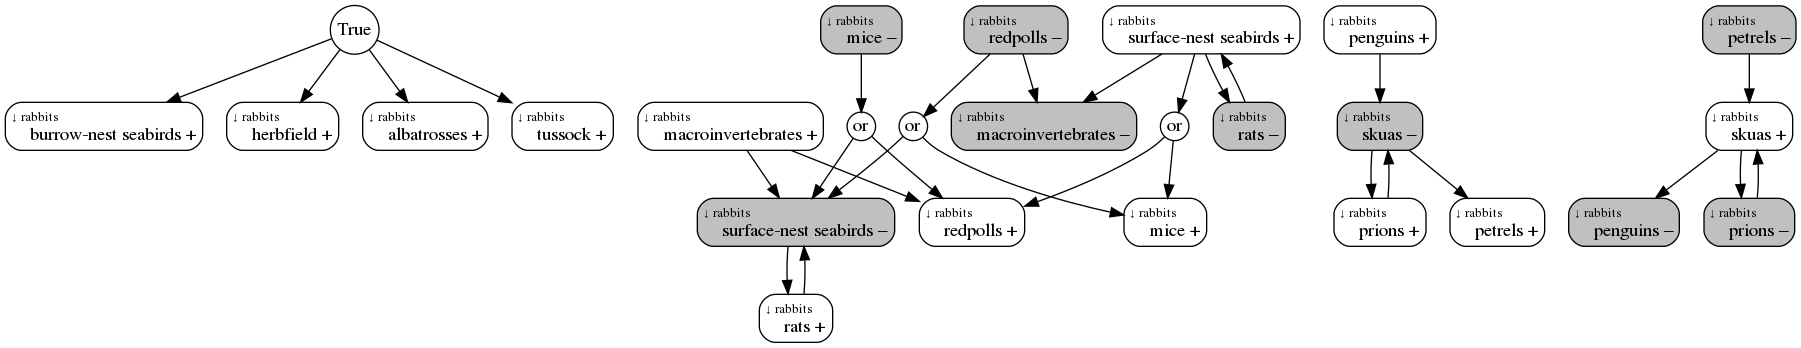
\includegraphics{uniques_web1_rabbits_pcus.png} Implication network.


    % Add a bibliography block to the postdoc
    
    
    
    \end{document}
